\documentclass[11pt]{article}
\usepackage[utf8]{inputenc}
\usepackage[dvips]{graphicx}
\usepackage{fancybox}
\usepackage{verbatim}
\usepackage{multirow,array}
\usepackage{latexsym}
\usepackage{alltt}
\usepackage{hyperref}
\usepackage{textcomp}
\usepackage{color}
\usepackage{amsmath}
\usepackage{amsfonts}
\usepackage{tikz}
\usepackage{float}
\usepackage[hmargin=3cm,vmargin=5.0cm]{geometry}
%\topmargin=0cm
\topmargin=-2cm
\addtolength{\textheight}{6.5cm}
\addtolength{\textwidth}{2.0cm}
%\setlength{\leftmargin}{-5cm}
\setlength{\oddsidemargin}{0.0cm}
\setlength{\evensidemargin}{0.0cm}


\begin{document}

\section*{Student Information } 
%Write your full name and id number between the colon and newline
%Put one empty space character after colon and before newline
Full Name : Deniz Koluaçık\\
Id Number : 2310274\\

% Write your answers below the section tags

\section*{Answer 1}
\subsection*{a)}
\begin{figure}[H]
    \centering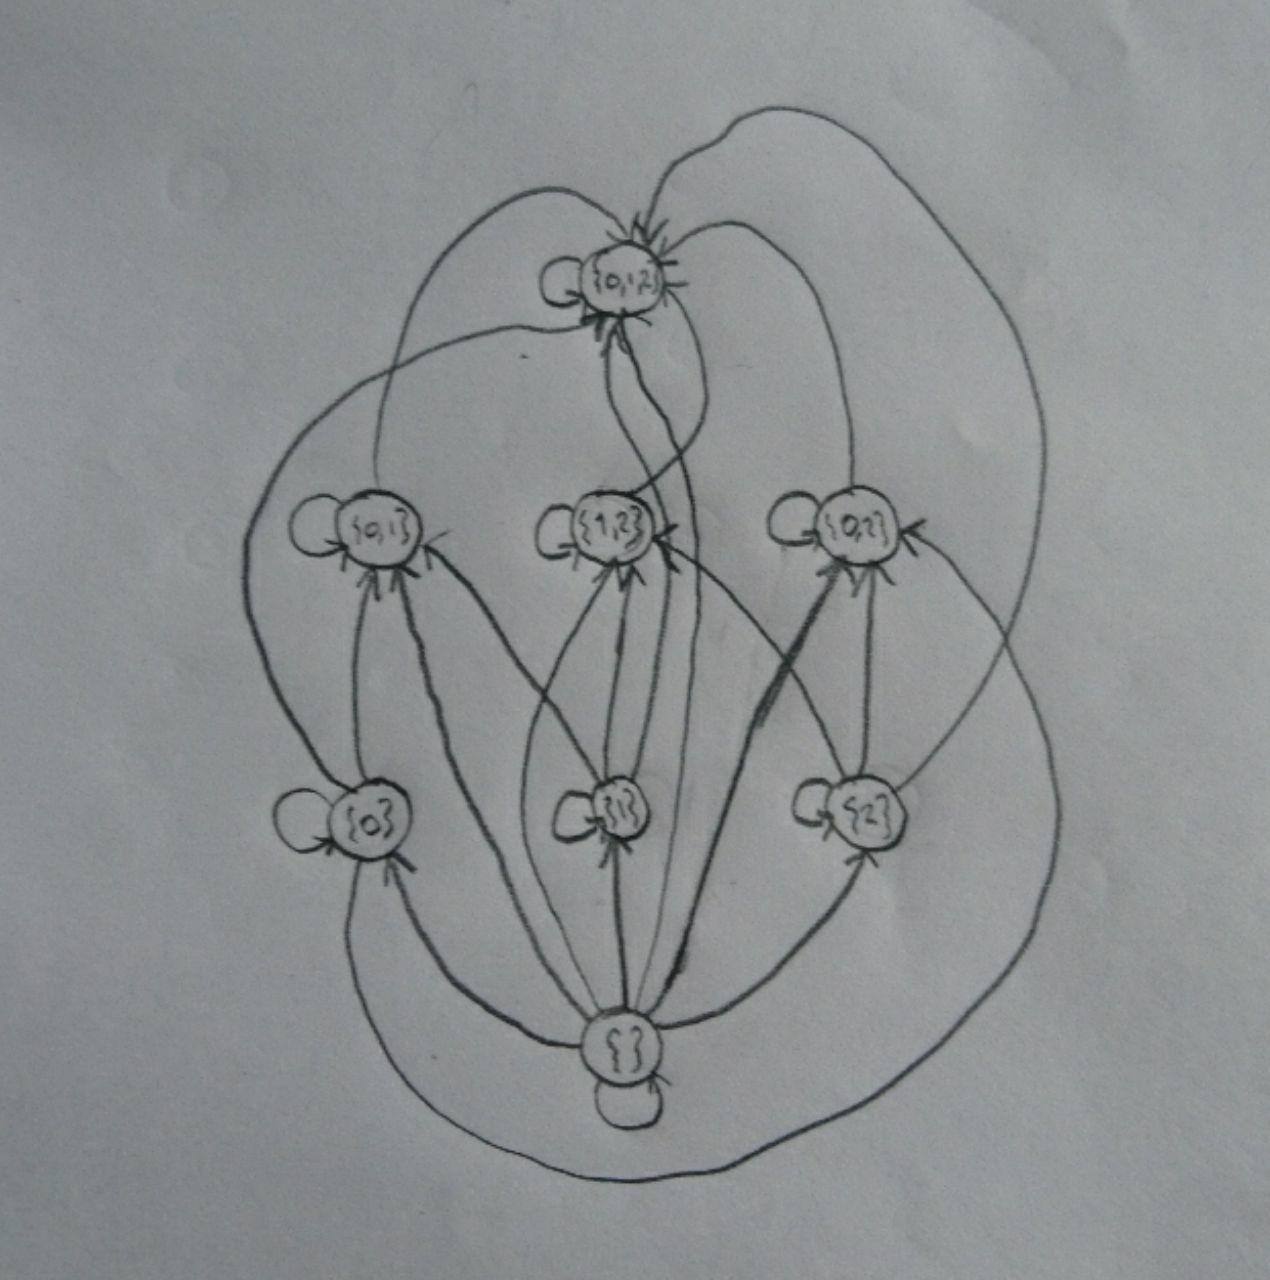
\includegraphics[width=0.5\textwidth]{digraph.jpg}
    \caption{R as a directed graph.}
    \label{fig:digraph}
\end{figure}
\subsection*{b)}
For the set $S$ together with the relation $R$ to be a \textit{poset}, $R$ needs to be a partial order. For that, $R$ needs to have three properties:

\begin{enumerate}
    \item{\textbf{Reflexive:}} All nodes on the directed graph depicted in figure \ref{fig:digraph} have a loop. Therefore, for any $x$ that is an element of the set $S$, $(x,x)$ is an element of $R$. Hence, $R$ is reflexive.
    \item{\textbf{Transitive:}} We need to show that $\forall x\forall y\forall z ( P(x,y) \land P(y,z) \rightarrow P(x,z))$ where $P(a,b)$ is true if and only if $(a,b) \in R$.\\
        By the definition of $R$, if $(x,y) \in R$, then $x \subseteq y$, similarly if $(y,z) \in R$, then $y \subseteq z$. If $x \subseteq y$ and $y \subseteq z$, then $x \subseteq z$. Hence, $(x,z) \in R$. Finally, since $(x,z)$ is also in $R$, $R$ is transitive.
    \item{\textbf{Antisymmetric:}} $(x \subseteq y) \land (y \subseteq x) \leftrightarrow (x = y)$. Similarly, $P(x,y) \land P(y,x) \leftrightarrow x = y$ where $P(a,b)$ is true if and only if $(a,b) \in R$. Therefore $R$ is antisymmetric.
\end{enumerate}
Since $R$ on $S$ is reflexive, transtive, and antisymmetric, $(S,R)$ is a poset.

\subsection*{c)}
For $(S,R)$ to be a total order every two element of $S$ needs to be comparable. As can be seen in figure \ref{fig:digraph}, neither $\{0\} \preceq \{1\}$ nor $\{1\} \preceq \{0\}$ is true, meaning that the two are not comparable. Hence, $(S,R)$ is not a total order.
\subsection*{d)}
\begin{figure}[H]
    \centering
    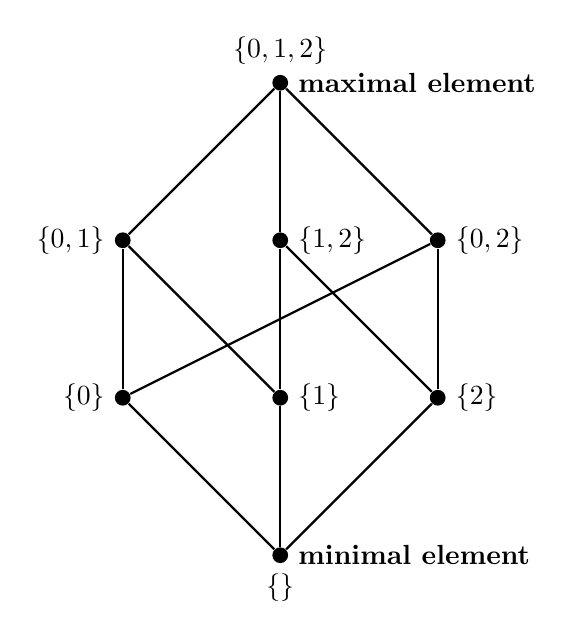
\begin{tikzpicture}
        \node[circle,fill,inner sep=2,minimum size=2mm,label={above:$\{0,1,2\}$},label={right:\textbf{maximal element}}] (0) at (2,6){};

        \node[circle,fill,inner sep=2,minimum size=2mm,label={left:$\{0,1\}$}] (1) at (0,4){};
        \node[circle,fill,inner sep=2,minimum size=2mm,label={right:$\{1,2\}$}] (2) at (2,4){};
        \node[circle,fill,inner sep=2,minimum size=2mm,label={right:$\{0,2\}$}] (3) at (4,4){};
        \node[circle,fill,inner sep=2,minimum size=2mm,label={left:$\{0\}$}] (4) at (0,2){};
        \node[circle,fill,inner sep=2,minimum size=2mm,label={right:$\{1\}$}] (5) at (2,2){};
        \node[circle,fill,inner sep=2,minimum size=2mm,label={right:$\{2\}$}] (6) at (4,2){};
        \node[circle,fill,inner sep=2,minimum size=2mm,label={below:$\{\}$},label={right:\textbf{minimal element}}] (7) at (2,0){};
        \path[-, thick] (7) edge (4);
        \path[-, thick] (7) edge (5);
        \path[-, thick] (7) edge (6);

        \path[-, thick] (6) edge (2);
        \path[-, thick] (6) edge (3);

        \path[-, thick] (5) edge (1);
        \path[-, thick] (5) edge (2);

        \path[-, thick] (4) edge (1);
        \path[-, thick] (4) edge (3);

        \path[-, thick] (1) edge (0);
        \path[-, thick] (2) edge (0);
        \path[-, thick] (3) edge (0);

    \end{tikzpicture}
    \caption{Hasse diagram for $(S,R)$.}
    \label{fig:hasse}
\end{figure}
\subsection*{e)} Consider the Hasse diagram in figure-\ref{fig:hasse}. For any two vertices $v$ and $w$, if they are comparable (if there is an edge $e$ incident to $v$ and $w$), there are two possible cases:
\begin{enumerate}
    \item $v \preceq w$: Since $v \preceq v$, $v$ is the greatest lower bound of the pair of these verices. Similarly, since $w \succeq w$, $w$ is the least upper bound.
    \item $w \preceq v$: Since $w \preceq w$, $w$ is the greatest lower bound of the pair of these verices. Similarly, since $v \succeq v$, $v$ is the least upper bound.
\end{enumerate}

If $v$ and $w$ are not comparable, then they are either of the same distance to the least element (their distances are either both two or both three), or one of them is of distance two while the other is of distance three to the least element.

\begin{enumerate}
    \item $v$ and $w$ are of same distance to the least vertice: Notice that for any pair of such vertices there is exactly one vertice that precedes them on the below, and there is exactly one vertice that succeeds them on the above. Those vertices are the greatest lower bound and the least upper bound, respectively.
    \item $v$ is of distance two to the least element, $w$ is of distance three: The greatest lower bound and the least upper bound are the least and the greatest elements, respectively.
\end{enumerate}

Finally, since for any pair of $v$ and $w$ there exists a least upper bound and a greatest lower bound, $(S,R)$ is a lattice.


\section*{Answer 2}
\subsection*{a)}

\begin{table}[H]
    \centering
    \begin{tabular}{c c}
        Initial vertex & Terminal vertex\\
        \hline
        a & \\
        b & a c\\
        c & f\\
        d & a c d e g\\
        e & c f g\\
        f & b\\
        g & d\\
    \end{tabular}
    \caption{adjacency list representation of $G$}
\end{table}

\subsection*{b)}
\begin{figure}[H]
    \centering
    $\begin{bmatrix} 
        0 & 0 & 0 & 0 & 0 & 0 & 0\\
        1 & 0 & 1 & 0 & 0 & 0 & 0\\
        0 & 0 & 0 & 0 & 0 & 1 & 0\\
        1 & 0 & 1 & 1 & 1 & 0 & 1\\
        0 & 0 & 1 & 0 & 0 & 1 & 1\\
        0 & 1 & 0 & 0 & 0 & 0 & 0\\
        0 & 0 & 0 & 1 & 0 & 0 & 0
    \end{bmatrix}$
    \caption{adjacency matrix representation of $G$}
\end{figure}

\subsection*{c)}

\begin{table}[H]
    \centering
    \begin{tabular}{*3{c}}
        & indegrees & outdegrees\\
        \hline
        a & 2 & 0 \\
        b & 1 & 2 \\
        c & 3 & 1 \\
        d & 2 & 5 \\
        e & 1 & 3 \\
        f & 2 & 1 \\
        g & 2 & 1 \\
    \end{tabular}
    \caption{indegrees and outdegrees of every vertex in $V$}
\end{table}


\subsection*{d)} \label{paths}
\begin{enumerate}
    \item $d,e,f,b,a$
    \item $d,e,f,b,c$
    \item $d,e,c,f,b$
    \item $e,g,d,c,f$
    \item $g,d,e,f,b$
    \item $g,d,c,f,b$
\end{enumerate}

\subsection*{e)}
\begin{enumerate}
    \item $d,e,g,d $
    \item $e,g,d,e $
    \item $g,d,e,g $
    \item $c,f,b,c $
    \item $f,b,c,f $
    \item $b,c,f,b $

\end{enumerate}

\subsection*{f)}
The outdegree the vertex $a$ is 0. There is no path from $a$ to any other vertex. Therefore, $G$ is not strongly-connected. 
Now, let $G'$ in figure-\ref{directedg} be the underlying undirected graph of $G$. Since, $G'$ is connected, $G$ is weakly-connected.

\begin{figure}[H]
    \centering
    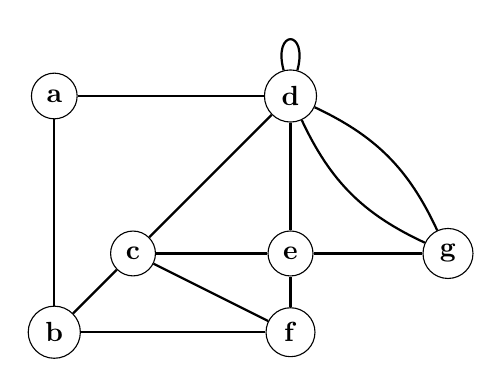
\begin{tikzpicture}[every loop/.style={}]

        \node[shape=circle,draw=black] (a) at (0, 3)     {\textbf{a}};
        \node[shape=circle,draw=black] (b) at (0, 0)     {\textbf{b}};
        \node[shape=circle,draw=black] (c) at (1, 1)     {\textbf{c}};
        \node[shape=circle,draw=black] (d) at (3, 3)     {\textbf{d}};
        \node[shape=circle,draw=black] (e) at (3, 1)     {\textbf{e}};
        \node[shape=circle,draw=black] (f) at (3, 0)     {\textbf{f}};
        \node[shape=circle,draw=black] (g) at (5, 1)     {\textbf{g}};

        \path[-, thick] (b) edge (a);
        \path[-, thick] (b) edge (c);
        \path[-, thick] (c) edge (f);
        \path[-, thick] (d) edge [loop above] (d);
        \path[-, thick] (d) edge (c);
        \path[-, thick] (d) edge (e);
        \path[-, thick] (d) edge (a);
        \path[-, thick] (d) edge [bend right=20] (g);
        \path[-, thick] (e) edge (c);
        \path[-, thick] (e) edge (f);
        \path[-, thick] (e) edge (g);
        \path[-, thick] (f) edge (b);
        \path[-, thick] (g) edge [bend right=20] (d);

    \end{tikzpicture} 
    \caption{The graph $G'$.} 
    \label{directedg}
\end{figure}

\subsection*{g)}
$G$ has three strongly-components, namely $G_1$, $G_2$, and $G_3$.\\
$G_1=(\{d,e,f\},\{(d,d),(d,e),(d,g),(e,g),(g,d)\})$\\
$G_2=(\{b,c,f\},\{(b,c),(c,f),(f,b)\})$\\
$G_3=(\{a\},\{\})$

\newpage
\subsection*{h)}
\begin{figure}[H]
	\centering
	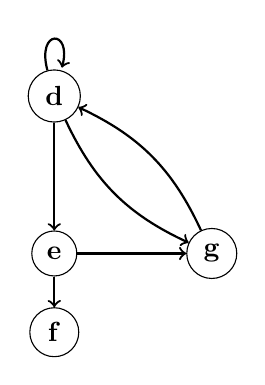
\begin{tikzpicture}
	
	\node[shape=circle,draw=black] (d) at (3, 3)     {\textbf{d}};
	\node[shape=circle,draw=black] (e) at (3, 1)     {\textbf{e}};
	\node[shape=circle,draw=black] (f) at (3, 0)     {\textbf{f}};
	\node[shape=circle,draw=black] (g) at (5, 1)     {\textbf{g}};

	\path[->, thick] (d) edge [loop above] (d);
	\path[->, thick] (d) edge (e);
	\path[->, thick] (d) edge [bend right=20] (g);
	\path[->, thick] (e) edge (f);
	\path[->, thick] (e) edge (g);
	\path[->, thick] (g) edge [bend right=20] (d);
	
	\end{tikzpicture} 
	\caption{The graph $H$}	
	\label{fig:H}
\end{figure}
Notice that we can use non-simple paths.
\begin{enumerate}
        \item $d,d,d,g$
        \item $d,d,e,g$
        \item $d,g,d,g$
\end{enumerate}
Three suchs paths exist.

\section*{Answer 3}
\begin{table}[H]
    \centering
    \begin{tabular}{cc}
        vertex & degree\\
        \hline
        \textbf{a} & 2\\
        \textbf{b} & 3\\
        \textbf{c} & 2\\
        \textbf{d} & 5\\
        \textbf{e} & 4\\
        \textbf{f} & 2\\
        \textbf{g} & 2\\
        \textbf{h} & 2\\
    \end{tabular}
    \caption{Degrees of vertices $G$ in Q3}
    \label{tab:degrees}
    
\end{table}
\subsection*{a)}
Since, connected graph $G$ has exactly two vertices of odd degree, by \textbf{Theorem 2 in page 697}, it has a Eular path.

\subsection*{b)}
Similarly, since, $G$ has vertices that has odd degrees, it has no Euler circuit by \textbf{Theorem 1 in page 696}.
\subsection*{c)}
Consider the path $c,b,a,d,e,f,g,h$. No vertex is visited twice and all vertices are visited. Therefore, $G$ has a Hamiltonian path.
\subsection*{d)}
No matter from which vertex we start, we have to visit the vertices $d$ and $e$ at least two times to traverse all vertices. Since there is always a non-starting-point-vertex that is visited two times, $G$ has no Hamiltonian circuit.


\section*{Answer 4}
\begin{table}[H]
    \centering
    \begin{tabular}{cc|cc}
        \multicolumn{2}{l|}{Graph $G$} & \multicolumn{2}{l}{Graph $G'$}\\
        \hline
        Vertex & Adjacent vertices & Vertex & Adjacent vertices\\
        \hline
         a & b e & a' & b' e' \\
         b & a c & b' & a' c' \\
         c & b d & c' & b' d' \\
         d & c e & d' & c' e' \\
         e & d a & e' & d' a' \\
    \end{tabular}
    \caption{adjacency list representations of $G$, and $G'$}
\end{table}
Clearly there is a one-to-one correspondance between the vertices of $G$ and $G'$, that is\\ $R=\{(a,a'),(b,b'),(c,c'),(d,d'),(e,e')\}$. Therefore, $G$ and $G'$ are isomorphic.


\section*{Answer 5}
\begin{figure}[H]
	\centering
	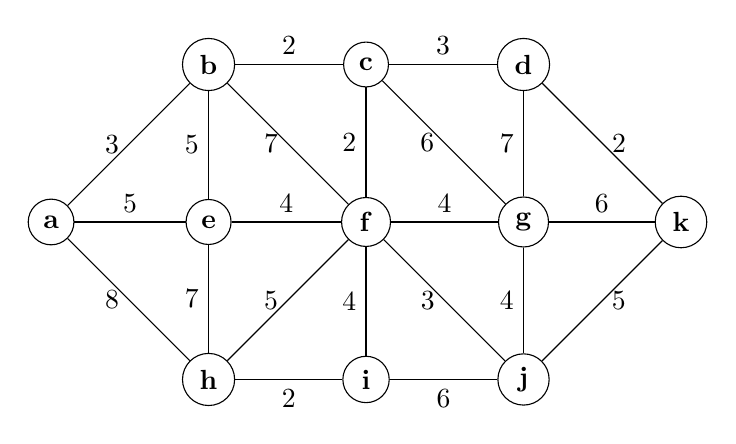
\begin{tikzpicture}
	\node[shape=circle,draw=black] (a) at (0, 2)     {\textbf{a}};
	\node[shape=circle,draw=black] (b) at (2, 4)     {\textbf{b}};
	\node[shape=circle,draw=black] (c) at (4, 4)     {\textbf{c}};
	\node[shape=circle,draw=black] (d) at (6, 4)     {\textbf{d}};
	\node[shape=circle,draw=black] (e) at (2, 2)     {\textbf{e}};
	\node[shape=circle,draw=black] (f) at (4, 2)     {\textbf{f}};
	\node[shape=circle,draw=black] (g) at (6, 2)     {\textbf{g}};
	\node[shape=circle,draw=black] (h) at (2, 0)     {\textbf{h}};
	\node[shape=circle,draw=black] (i) at (4, 0)     {\textbf{i}};
	\node[shape=circle,draw=black] (j) at (6, 0)     {\textbf{j}};
	\node[shape=circle,draw=black] (k) at (8, 2)     {\textbf{k}};

	\path[-] (a) edge node[left]{3} (b);
	\path[-] (a) edge node[above]{5} (e);
	\path[-] (a) edge node[left]{8} (h);
	\path[-] (b) edge node[left]{5} (e);
	\path[-] (b) edge node[left]{7} (f);
	\path[-] (b) edge node[above]{2} (c);
	\path[-] (e) edge node[above]{4} (f);
	\path[-] (e) edge node[left]{7} (h);
	\path[-] (h) edge node[left]{5} (f);	
	\path[-] (h) edge node[below]{2} (i);	
	\path[-] (c) edge node[above]{3} (d);
	\path[-] (c) edge node[left]{6} (g);
	\path[-] (c) edge node[left]{2} (f);
	\path[-] (f) edge node[above]{4} (g);
	\path[-] (f) edge node[left]{3} (j);
	\path[-] (f) edge node[left]{4} (i);
	\path[-] (i) edge node[below]{6} (j);	
	\path[-] (d) edge node[right]{2} (k);
	\path[-] (d) edge node[left]{7} (g);
	\path[-] (g) edge node[above]{6} (k);
	\path[-] (g) edge node[left]{4} (j);
	\path[-] (j) edge node[right]{5} (k);
		
	\end{tikzpicture} 
	\caption{Graph $G$ in Q5.}
	\label{orig}
\end{figure}
\subsection*{a)}

\begin{figure}[H]
	\centering
	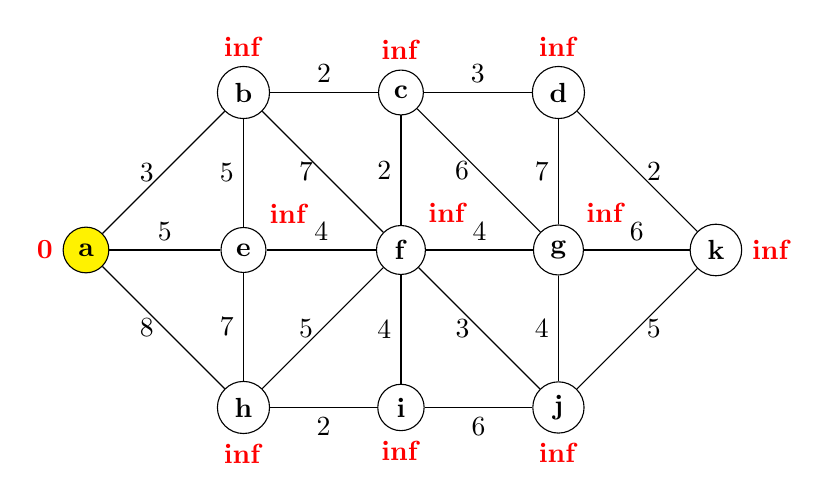
\begin{tikzpicture}
        \node[shape=circle,draw=black,fill=yellow,label={left:\color{red}\textbf{0}}] (a) at (0, 2)     {\textbf{a}};
        \node[shape=circle,draw=black,label={above:\color{red}\textbf{inf}}] (b) at (2, 4)     {\textbf{b}};
        \node[shape=circle,draw=black,label={above:\color{red}\textbf{inf}}] (c) at (4, 4)     {\textbf{c}};
        \node[shape=circle,draw=black,label={above:\color{red}\textbf{inf}}] (d) at (6, 4)     {\textbf{d}};
        \node[shape=circle,draw=black,label={above right:\color{red}\textbf{inf}}] (e) at (2, 2)     {\textbf{e}};
        \node[shape=circle,draw=black,label={above right:\color{red}\textbf{inf}}] (f) at (4, 2)     {\textbf{f}};
        \node[shape=circle,draw=black,label={above right:\color{red}\textbf{inf}}] (g) at (6, 2)     {\textbf{g}};
        \node[shape=circle,draw=black,label={below:\color{red}\textbf{inf}}] (h) at (2, 0)     {\textbf{h}};
        \node[shape=circle,draw=black,label={below:\color{red}\textbf{inf}}] (i) at (4, 0)     {\textbf{i}};
        \node[shape=circle,draw=black,label={below:\color{red}\textbf{inf}}] (j) at (6, 0)     {\textbf{j}};
        \node[shape=circle,draw=black,label={right:\color{red}\textbf{inf}}] (k) at (8, 2)     {\textbf{k}};

	\path[-] (a) edge node[left]{3} (b);
	\path[-] (a) edge node[above]{5} (e);
	\path[-] (a) edge node[left]{8} (h);
	\path[-] (b) edge node[left]{5} (e);
	\path[-] (b) edge node[left]{7} (f);
	\path[-] (b) edge node[above]{2} (c);
	\path[-] (e) edge node[above]{4} (f);
	\path[-] (e) edge node[left]{7} (h);
	\path[-] (h) edge node[left]{5} (f);	
	\path[-] (h) edge node[below]{2} (i);	
	\path[-] (c) edge node[above]{3} (d);
	\path[-] (c) edge node[left]{6} (g);
	\path[-] (c) edge node[left]{2} (f);
	\path[-] (f) edge node[above]{4} (g);
	\path[-] (f) edge node[left]{3} (j);
	\path[-] (f) edge node[left]{4} (i);
	\path[-] (i) edge node[below]{6} (j);	
	\path[-] (d) edge node[right]{2} (k);
	\path[-] (d) edge node[left]{7} (g);
	\path[-] (g) edge node[above]{6} (k);
	\path[-] (g) edge node[left]{4} (j);
	\path[-] (j) edge node[right]{5} (k);
	\end{tikzpicture} 
	\caption{Assign tentative distance for all vertices.}
\end{figure}

\begin{figure}[H]
	\centering
	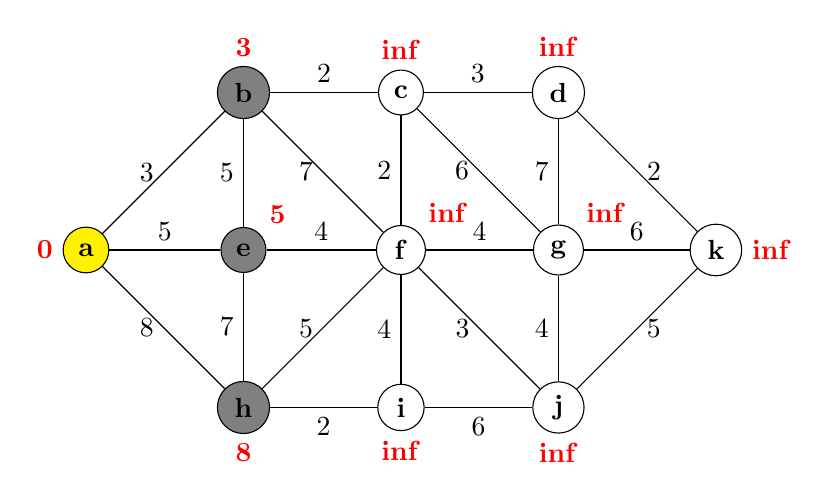
\begin{tikzpicture}
        \node[shape=circle,draw=black,fill=yellow,label={left:\color{red}\textbf{0}}] (a) at (0, 2)     {\textbf{a}};
        \node[shape=circle,draw=black,fill=gray,label={above:\color{red}\textbf{3}}] (b) at (2, 4)     {\textbf{b}};
        \node[shape=circle,draw=black,label={above:\color{red}\textbf{inf}}] (c) at (4, 4)     {\textbf{c}};
        \node[shape=circle,draw=black,label={above:\color{red}\textbf{inf}}] (d) at (6, 4)     {\textbf{d}};
        \node[shape=circle,draw=black,fill=gray,label={above right:\color{red}\textbf{5}}] (e) at (2, 2)     {\textbf{e}};
        \node[shape=circle,draw=black,label={above right:\color{red}\textbf{inf}}] (f) at (4, 2)     {\textbf{f}};
        \node[shape=circle,draw=black,label={above right:\color{red}\textbf{inf}}] (g) at (6, 2)     {\textbf{g}};
        \node[shape=circle,draw=black,fill=gray,label={below:\color{red}\textbf{8}}] (h) at (2, 0)     {\textbf{h}};
        \node[shape=circle,draw=black,label={below:\color{red}\textbf{inf}}] (i) at (4, 0)     {\textbf{i}};
        \node[shape=circle,draw=black,label={below:\color{red}\textbf{inf}}] (j) at (6, 0)     {\textbf{j}};
        \node[shape=circle,draw=black,label={right:\color{red}\textbf{inf}}] (k) at (8, 2)     {\textbf{k}};

	\path[-] (a) edge node[left]{3} (b);
	\path[-] (a) edge node[above]{5} (e);
	\path[-] (a) edge node[left]{8} (h);
	\path[-] (b) edge node[left]{5} (e);
	\path[-] (b) edge node[left]{7} (f);
	\path[-] (b) edge node[above]{2} (c);
	\path[-] (e) edge node[above]{4} (f);
	\path[-] (e) edge node[left]{7} (h);
	\path[-] (h) edge node[left]{5} (f);	
	\path[-] (h) edge node[below]{2} (i);	
	\path[-] (c) edge node[above]{3} (d);
	\path[-] (c) edge node[left]{6} (g);
	\path[-] (c) edge node[left]{2} (f);
	\path[-] (f) edge node[above]{4} (g);
	\path[-] (f) edge node[left]{3} (j);
	\path[-] (f) edge node[left]{4} (i);
	\path[-] (i) edge node[below]{6} (j);	
	\path[-] (d) edge node[right]{2} (k);
	\path[-] (d) edge node[left]{7} (g);
	\path[-] (g) edge node[above]{6} (k);
	\path[-] (g) edge node[left]{4} (j);
	\path[-] (j) edge node[right]{5} (k);
	\end{tikzpicture} 
	\caption{Check all unvisited neighboring vertices of the current node.}
\end{figure}

\begin{figure}[H]
	\centering
	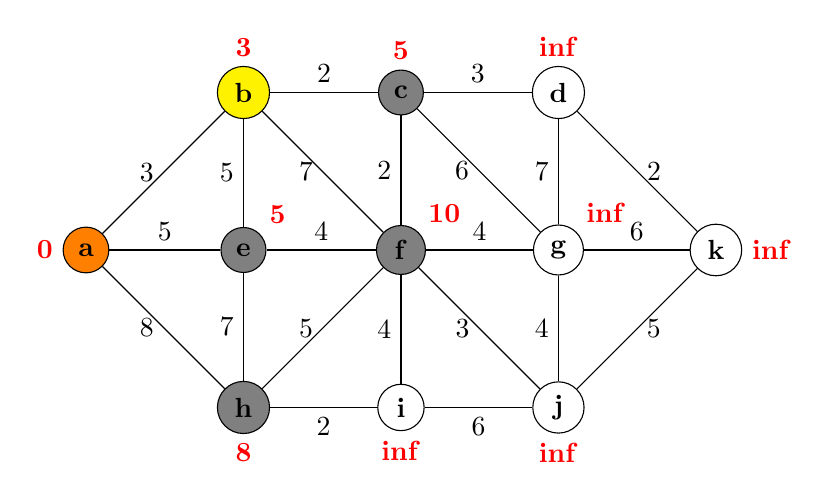
\begin{tikzpicture}
        \node[shape=circle,draw=black,fill=orange,label={left:\color{red}{\textbf{0}}}] (a) at (0, 2)     {\textbf{a}};
        \node[shape=circle,draw=black,fill=yellow,label={above:\color{red}\textbf{3}}] (b) at (2, 4)     {\textbf{b}};
        \node[shape=circle,draw=black,fill=gray,label={above:\color{red}\textbf{5}}] (c) at (4, 4)     {\textbf{c}};
        \node[shape=circle,draw=black,label={above:\color{red}\textbf{inf}}] (d) at (6, 4)     {\textbf{d}};
        \node[shape=circle,draw=black,fill=gray,label={above right:\color{red}\textbf{5}}] (e) at (2, 2)     {\textbf{e}};
        \node[shape=circle,draw=black,fill=gray,label={above right:\color{red}\textbf{10}}] (f) at (4, 2)     {\textbf{f}};
        \node[shape=circle,draw=black,label={above right:\color{red}\textbf{inf}}] (g) at (6, 2)     {\textbf{g}};
        \node[shape=circle,draw=black,fill=gray,label={below:\color{red}\textbf{8}}] (h) at (2, 0)     {\textbf{h}};
        \node[shape=circle,draw=black,label={below:\color{red}\textbf{inf}}] (i) at (4, 0)     {\textbf{i}};
        \node[shape=circle,draw=black,label={below:\color{red}\textbf{inf}}] (j) at (6, 0)     {\textbf{j}};
        \node[shape=circle,draw=black,label={right:\color{red}\textbf{inf}}] (k) at (8, 2)     {\textbf{k}};

	\path[-] (a) edge node[left]{3} (b);
	\path[-] (a) edge node[above]{5} (e);
	\path[-] (a) edge node[left]{8} (h);
	\path[-] (b) edge node[left]{5} (e);
	\path[-] (b) edge node[left]{7} (f);
	\path[-] (b) edge node[above]{2} (c);
	\path[-] (e) edge node[above]{4} (f);
	\path[-] (e) edge node[left]{7} (h);
	\path[-] (h) edge node[left]{5} (f);	
	\path[-] (h) edge node[below]{2} (i);	
	\path[-] (c) edge node[above]{3} (d);
	\path[-] (c) edge node[left]{6} (g);
	\path[-] (c) edge node[left]{2} (f);
	\path[-] (f) edge node[above]{4} (g);
	\path[-] (f) edge node[left]{3} (j);
	\path[-] (f) edge node[left]{4} (i);
	\path[-] (i) edge node[below]{6} (j);	
	\path[-] (d) edge node[right]{2} (k);
	\path[-] (d) edge node[left]{7} (g);
	\path[-] (g) edge node[above]{6} (k);
	\path[-] (g) edge node[left]{4} (j);
	\path[-] (j) edge node[right]{5} (k);
	\end{tikzpicture} 
	\caption{Move on to the vertex with the least distance to the initial vertex.}
\end{figure}

\begin{figure}[H]
	\centering
	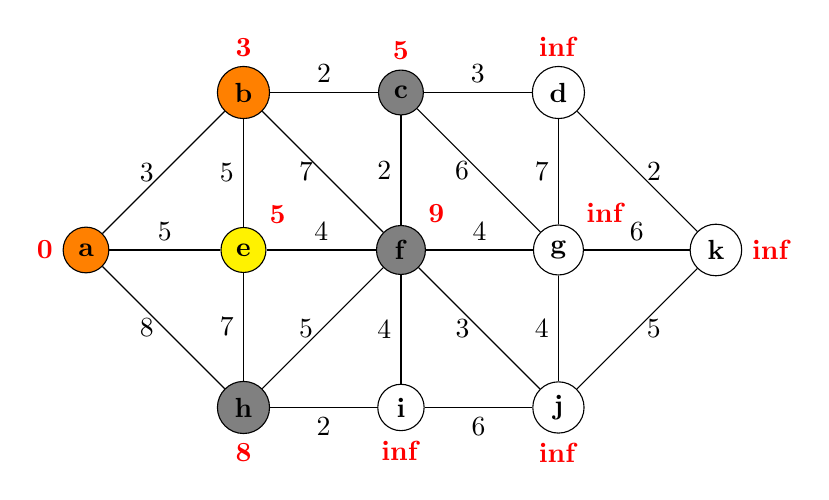
\begin{tikzpicture}
        \node[shape=circle,draw=black,fill=orange,label={left:\color{red}{\textbf{0}}}] (a) at (0, 2)     {\textbf{a}};
        \node[shape=circle,draw=black,fill=orange,label={above:\color{red}\textbf{3}}] (b) at (2, 4)     {\textbf{b}};
        \node[shape=circle,draw=black,fill=gray,label={above:\color{red}\textbf{5}}] (c) at (4, 4)     {\textbf{c}};
        \node[shape=circle,draw=black,label={above:\color{red}\textbf{inf}}] (d) at (6, 4)     {\textbf{d}};
        \node[shape=circle,draw=black,fill=yellow,label={above right:\color{red}\textbf{5}}] (e) at (2, 2)     {\textbf{e}};
        \node[shape=circle,draw=black,fill=gray,label={above right:\color{red}\textbf{9}}] (f) at (4, 2)     {\textbf{f}};
        \node[shape=circle,draw=black,label={above right:\color{red}\textbf{inf}}] (g) at (6, 2)     {\textbf{g}};
        \node[shape=circle,draw=black,fill=gray,label={below:\color{red}\textbf{8}}] (h) at (2, 0)     {\textbf{h}};
        \node[shape=circle,draw=black,label={below:\color{red}\textbf{inf}}] (i) at (4, 0)     {\textbf{i}};
        \node[shape=circle,draw=black,label={below:\color{red}\textbf{inf}}] (j) at (6, 0)     {\textbf{j}};
        \node[shape=circle,draw=black,label={right:\color{red}\textbf{inf}}] (k) at (8, 2)     {\textbf{k}};

	\path[-] (a) edge node[left]{3} (b);
	\path[-] (a) edge node[above]{5} (e);
	\path[-] (a) edge node[left]{8} (h);
	\path[-] (b) edge node[left]{5} (e);
	\path[-] (b) edge node[left]{7} (f);
	\path[-] (b) edge node[above]{2} (c);
	\path[-] (e) edge node[above]{4} (f);
	\path[-] (e) edge node[left]{7} (h);
	\path[-] (h) edge node[left]{5} (f);	
	\path[-] (h) edge node[below]{2} (i);	
	\path[-] (c) edge node[above]{3} (d);
	\path[-] (c) edge node[left]{6} (g);
	\path[-] (c) edge node[left]{2} (f);
	\path[-] (f) edge node[above]{4} (g);
	\path[-] (f) edge node[left]{3} (j);
	\path[-] (f) edge node[left]{4} (i);
	\path[-] (i) edge node[below]{6} (j);	
	\path[-] (d) edge node[right]{2} (k);
	\path[-] (d) edge node[left]{7} (g);
	\path[-] (g) edge node[above]{6} (k);
	\path[-] (g) edge node[left]{4} (j);
	\path[-] (j) edge node[right]{5} (k);
	\end{tikzpicture} 
	\caption{Repeat the previous step for vertex $e$.}
\end{figure}

\begin{figure}[H]
	\centering
	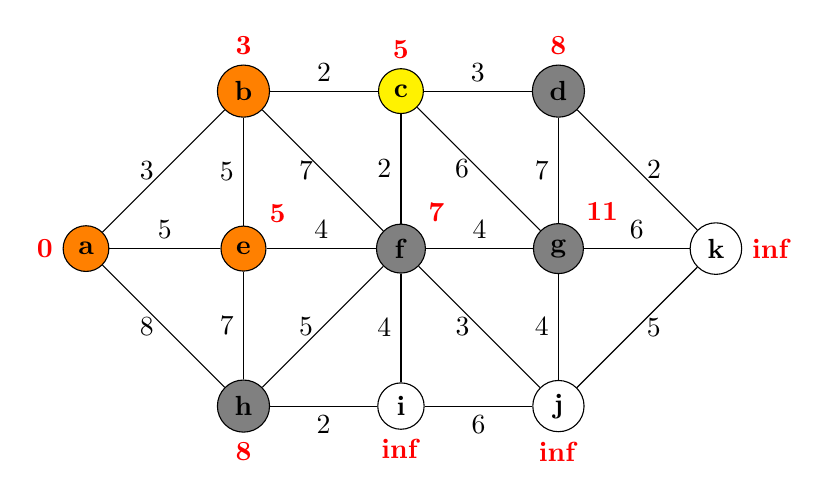
\begin{tikzpicture}
        \node[shape=circle,draw=black,fill=orange,label={left:\color{red}{\textbf{0}}}] (a) at (0, 2)     {\textbf{a}};
        \node[shape=circle,draw=black,fill=orange,label={above:\color{red}\textbf{3}}] (b) at (2, 4)     {\textbf{b}};
        \node[shape=circle,draw=black,fill=yellow,label={above:\color{red}\textbf{5}}] (c) at (4, 4)     {\textbf{c}};
        \node[shape=circle,draw=black,fill=gray,label={above:\color{red}\textbf{8}}] (d) at (6, 4)     {\textbf{d}};
        \node[shape=circle,draw=black,fill=orange,label={above right:\color{red}\textbf{5}}] (e) at (2, 2)     {\textbf{e}};
        \node[shape=circle,draw=black,fill=gray,label={above right:\color{red}\textbf{7}}] (f) at (4, 2)     {\textbf{f}};
        \node[shape=circle,draw=black,fill=gray,label={above right:\color{red}\textbf{11}}] (g) at (6, 2)     {\textbf{g}};
        \node[shape=circle,draw=black,fill=gray,label={below:\color{red}\textbf{8}}] (h) at (2, 0)     {\textbf{h}};
        \node[shape=circle,draw=black,label={below:\color{red}\textbf{inf}}] (i) at (4, 0)     {\textbf{i}};
        \node[shape=circle,draw=black,label={below:\color{red}\textbf{inf}}] (j) at (6, 0)     {\textbf{j}};
        \node[shape=circle,draw=black,label={right:\color{red}\textbf{inf}}] (k) at (8, 2)     {\textbf{k}};

	\path[-] (a) edge node[left]{3} (b);
	\path[-] (a) edge node[above]{5} (e);
	\path[-] (a) edge node[left]{8} (h);
	\path[-] (b) edge node[left]{5} (e);
	\path[-] (b) edge node[left]{7} (f);
	\path[-] (b) edge node[above]{2} (c);
	\path[-] (e) edge node[above]{4} (f);
	\path[-] (e) edge node[left]{7} (h);
	\path[-] (h) edge node[left]{5} (f);	
	\path[-] (h) edge node[below]{2} (i);	
	\path[-] (c) edge node[above]{3} (d);
	\path[-] (c) edge node[left]{6} (g);
	\path[-] (c) edge node[left]{2} (f);
	\path[-] (f) edge node[above]{4} (g);
	\path[-] (f) edge node[left]{3} (j);
	\path[-] (f) edge node[left]{4} (i);
	\path[-] (i) edge node[below]{6} (j);	
	\path[-] (d) edge node[right]{2} (k);
	\path[-] (d) edge node[left]{7} (g);
	\path[-] (g) edge node[above]{6} (k);
	\path[-] (g) edge node[left]{4} (j);
	\path[-] (j) edge node[right]{5} (k);
	\end{tikzpicture} 
	\caption{Repeat the previous step for vertex $c$.}
\end{figure}

\begin{figure}[H]
	\centering
	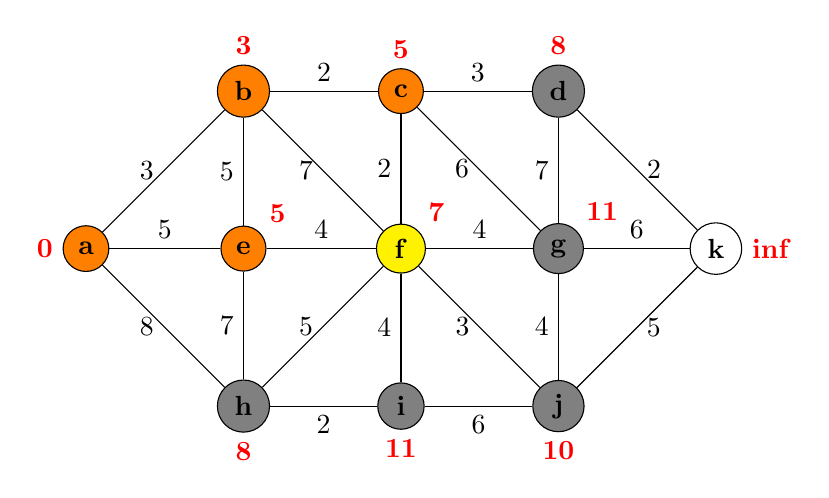
\begin{tikzpicture}
        \node[shape=circle,draw=black,fill=orange,label={left:\color{red}{\textbf{0}}}] (a) at (0, 2)     {\textbf{a}};
        \node[shape=circle,draw=black,fill=orange,label={above:\color{red}\textbf{3}}] (b) at (2, 4)     {\textbf{b}};
        \node[shape=circle,draw=black,fill=orange,label={above:\color{red}\textbf{5}}] (c) at (4, 4)     {\textbf{c}};
        \node[shape=circle,draw=black,fill=gray,label={above:\color{red}\textbf{8}}] (d) at (6, 4)     {\textbf{d}};
        \node[shape=circle,draw=black,fill=orange,label={above right:\color{red}\textbf{5}}] (e) at (2, 2)     {\textbf{e}};
        \node[shape=circle,draw=black,fill=yellow,label={above right:\color{red}\textbf{7}}] (f) at (4, 2)     {\textbf{f}};
        \node[shape=circle,draw=black,fill=gray,label={above right:\color{red}\textbf{11}}] (g) at (6, 2)     {\textbf{g}};
        \node[shape=circle,draw=black,fill=gray,label={below:\color{red}\textbf{8}}] (h) at (2, 0)     {\textbf{h}};
        \node[shape=circle,draw=black,fill=gray,label={below:\color{red}\textbf{11}}] (i) at (4, 0)     {\textbf{i}};
        \node[shape=circle,draw=black,fill=gray,label={below:\color{red}\textbf{10}}] (j) at (6, 0)     {\textbf{j}};
        \node[shape=circle,draw=black,label={right:\color{red}\textbf{inf}}] (k) at (8, 2)     {\textbf{k}};

	\path[-] (a) edge node[left]{3} (b);
	\path[-] (a) edge node[above]{5} (e);
	\path[-] (a) edge node[left]{8} (h);
	\path[-] (b) edge node[left]{5} (e);
	\path[-] (b) edge node[left]{7} (f);
	\path[-] (b) edge node[above]{2} (c);
	\path[-] (e) edge node[above]{4} (f);
	\path[-] (e) edge node[left]{7} (h);
	\path[-] (h) edge node[left]{5} (f);	
	\path[-] (h) edge node[below]{2} (i);	
	\path[-] (c) edge node[above]{3} (d);
	\path[-] (c) edge node[left]{6} (g);
	\path[-] (c) edge node[left]{2} (f);
	\path[-] (f) edge node[above]{4} (g);
	\path[-] (f) edge node[left]{3} (j);
	\path[-] (f) edge node[left]{4} (i);
	\path[-] (i) edge node[below]{6} (j);	
	\path[-] (d) edge node[right]{2} (k);
	\path[-] (d) edge node[left]{7} (g);
	\path[-] (g) edge node[above]{6} (k);
	\path[-] (g) edge node[left]{4} (j);
	\path[-] (j) edge node[right]{5} (k);
	\end{tikzpicture} 
	\caption{Repeat the previous step for vertex $f$.}
\end{figure}

\begin{figure}[H]
	\centering
	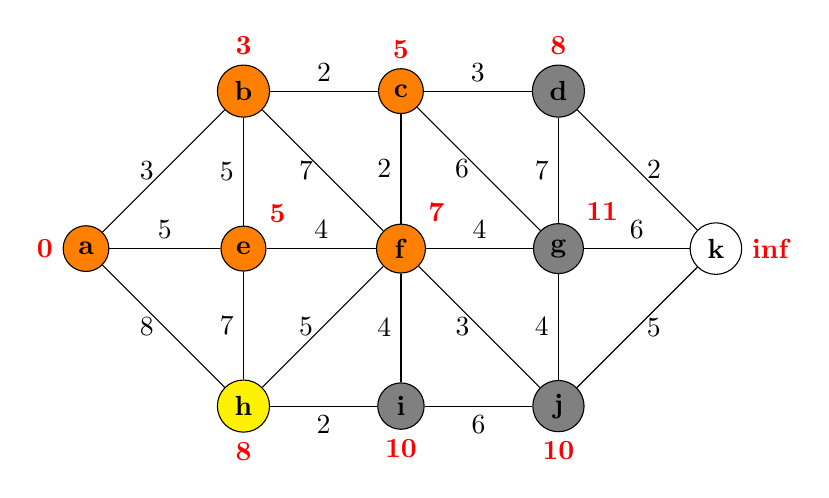
\begin{tikzpicture}
        \node[shape=circle,draw=black,fill=orange,label={left:\color{red}{\textbf{0}}}] (a) at (0, 2)     {\textbf{a}};
        \node[shape=circle,draw=black,fill=orange,label={above:\color{red}\textbf{3}}] (b) at (2, 4)     {\textbf{b}};
        \node[shape=circle,draw=black,fill=orange,label={above:\color{red}\textbf{5}}] (c) at (4, 4)     {\textbf{c}};
        \node[shape=circle,draw=black,fill=gray,label={above:\color{red}\textbf{8}}] (d) at (6, 4)     {\textbf{d}};
        \node[shape=circle,draw=black,fill=orange,label={above right:\color{red}\textbf{5}}] (e) at (2, 2)     {\textbf{e}};
        \node[shape=circle,draw=black,fill=orange,label={above right:\color{red}\textbf{7}}] (f) at (4, 2)     {\textbf{f}};
        \node[shape=circle,draw=black,fill=gray,label={above right:\color{red}\textbf{11}}] (g) at (6, 2)     {\textbf{g}};
        \node[shape=circle,draw=black,fill=yellow,label={below:\color{red}\textbf{8}}] (h) at (2, 0)     {\textbf{h}};
        \node[shape=circle,draw=black,fill=gray,label={below:\color{red}\textbf{10}}] (i) at (4, 0)     {\textbf{i}};
        \node[shape=circle,draw=black,fill=gray,label={below:\color{red}\textbf{10}}] (j) at (6, 0)     {\textbf{j}};
        \node[shape=circle,draw=black,label={right:\color{red}\textbf{inf}}] (k) at (8, 2)     {\textbf{k}};

	\path[-] (a) edge node[left]{3} (b);
	\path[-] (a) edge node[above]{5} (e);
	\path[-] (a) edge node[left]{8} (h);
	\path[-] (b) edge node[left]{5} (e);
	\path[-] (b) edge node[left]{7} (f);
	\path[-] (b) edge node[above]{2} (c);
	\path[-] (e) edge node[above]{4} (f);
	\path[-] (e) edge node[left]{7} (h);
	\path[-] (h) edge node[left]{5} (f);	
	\path[-] (h) edge node[below]{2} (i);	
	\path[-] (c) edge node[above]{3} (d);
	\path[-] (c) edge node[left]{6} (g);
	\path[-] (c) edge node[left]{2} (f);
	\path[-] (f) edge node[above]{4} (g);
	\path[-] (f) edge node[left]{3} (j);
	\path[-] (f) edge node[left]{4} (i);
	\path[-] (i) edge node[below]{6} (j);	
	\path[-] (d) edge node[right]{2} (k);
	\path[-] (d) edge node[left]{7} (g);
	\path[-] (g) edge node[above]{6} (k);
	\path[-] (g) edge node[left]{4} (j);
	\path[-] (j) edge node[right]{5} (k);
	\end{tikzpicture} 
	\caption{Repeat the previous step for vertex $h$.}
\end{figure}

\begin{figure}[H]
	\centering
	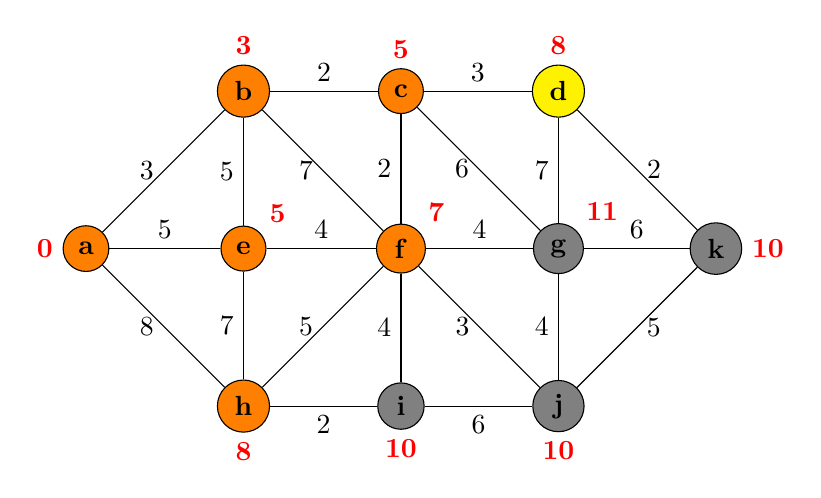
\begin{tikzpicture}
        \node[shape=circle,draw=black,fill=orange,label={left:\color{red}{\textbf{0}}}] (a) at (0, 2)     {\textbf{a}};
        \node[shape=circle,draw=black,fill=orange,label={above:\color{red}\textbf{3}}] (b) at (2, 4)     {\textbf{b}};
        \node[shape=circle,draw=black,fill=orange,label={above:\color{red}\textbf{5}}] (c) at (4, 4)     {\textbf{c}};
        \node[shape=circle,draw=black,fill=yellow,label={above:\color{red}\textbf{8}}] (d) at (6, 4)     {\textbf{d}};
        \node[shape=circle,draw=black,fill=orange,label={above right:\color{red}\textbf{5}}] (e) at (2, 2)     {\textbf{e}};
        \node[shape=circle,draw=black,fill=orange,label={above right:\color{red}\textbf{7}}] (f) at (4, 2)     {\textbf{f}};
        \node[shape=circle,draw=black,fill=gray,label={above right:\color{red}\textbf{11}}] (g) at (6, 2)     {\textbf{g}};
        \node[shape=circle,draw=black,fill=orange,label={below:\color{red}\textbf{8}}] (h) at (2, 0)     {\textbf{h}};
        \node[shape=circle,draw=black,fill=gray,label={below:\color{red}\textbf{10}}] (i) at (4, 0)     {\textbf{i}};
        \node[shape=circle,draw=black,fill=gray,label={below:\color{red}\textbf{10}}] (j) at (6, 0)     {\textbf{j}};
        \node[shape=circle,draw=black,fill=gray,label={right:\color{red}\textbf{10}}] (k) at (8, 2)     {\textbf{k}};

	\path[-] (a) edge node[left]{3} (b);
	\path[-] (a) edge node[above]{5} (e);
	\path[-] (a) edge node[left]{8} (h);
	\path[-] (b) edge node[left]{5} (e);
	\path[-] (b) edge node[left]{7} (f);
	\path[-] (b) edge node[above]{2} (c);
	\path[-] (e) edge node[above]{4} (f);
	\path[-] (e) edge node[left]{7} (h);
	\path[-] (h) edge node[left]{5} (f);	
	\path[-] (h) edge node[below]{2} (i);	
	\path[-] (c) edge node[above]{3} (d);
	\path[-] (c) edge node[left]{6} (g);
	\path[-] (c) edge node[left]{2} (f);
	\path[-] (f) edge node[above]{4} (g);
	\path[-] (f) edge node[left]{3} (j);
	\path[-] (f) edge node[left]{4} (i);
	\path[-] (i) edge node[below]{6} (j);	
	\path[-] (d) edge node[right]{2} (k);
	\path[-] (d) edge node[left]{7} (g);
	\path[-] (g) edge node[above]{6} (k);
	\path[-] (g) edge node[left]{4} (j);
	\path[-] (j) edge node[right]{5} (k);
	\end{tikzpicture} 
	\caption{Repeat the previous step for vertex $d$.}
\end{figure}

\begin{figure}[H]
	\centering
	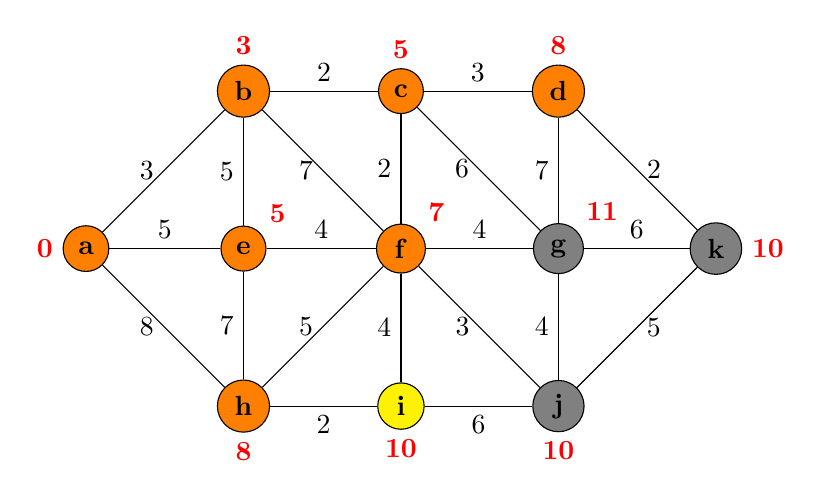
\begin{tikzpicture}
        \node[shape=circle,draw=black,fill=orange,label={left:\color{red}{\textbf{0}}}] (a) at (0, 2)     {\textbf{a}};
        \node[shape=circle,draw=black,fill=orange,label={above:\color{red}\textbf{3}}] (b) at (2, 4)     {\textbf{b}};
        \node[shape=circle,draw=black,fill=orange,label={above:\color{red}\textbf{5}}] (c) at (4, 4)     {\textbf{c}};
        \node[shape=circle,draw=black,fill=orange,label={above:\color{red}\textbf{8}}] (d) at (6, 4)     {\textbf{d}};
        \node[shape=circle,draw=black,fill=orange,label={above right:\color{red}\textbf{5}}] (e) at (2, 2)     {\textbf{e}};
        \node[shape=circle,draw=black,fill=orange,label={above right:\color{red}\textbf{7}}] (f) at (4, 2)     {\textbf{f}};
        \node[shape=circle,draw=black,fill=gray,label={above right:\color{red}\textbf{11}}] (g) at (6, 2)     {\textbf{g}};
        \node[shape=circle,draw=black,fill=orange,label={below:\color{red}\textbf{8}}] (h) at (2, 0)     {\textbf{h}};
        \node[shape=circle,draw=black,fill=yellow,label={below:\color{red}\textbf{10}}] (i) at (4, 0)     {\textbf{i}};
        \node[shape=circle,draw=black,fill=gray,label={below:\color{red}\textbf{10}}] (j) at (6, 0)     {\textbf{j}};
        \node[shape=circle,draw=black,fill=gray,label={right:\color{red}\textbf{10}}] (k) at (8, 2)     {\textbf{k}};

	\path[-] (a) edge node[left]{3} (b);
	\path[-] (a) edge node[above]{5} (e);
	\path[-] (a) edge node[left]{8} (h);
	\path[-] (b) edge node[left]{5} (e);
	\path[-] (b) edge node[left]{7} (f);
	\path[-] (b) edge node[above]{2} (c);
	\path[-] (e) edge node[above]{4} (f);
	\path[-] (e) edge node[left]{7} (h);
	\path[-] (h) edge node[left]{5} (f);	
	\path[-] (h) edge node[below]{2} (i);	
	\path[-] (c) edge node[above]{3} (d);
	\path[-] (c) edge node[left]{6} (g);
	\path[-] (c) edge node[left]{2} (f);
	\path[-] (f) edge node[above]{4} (g);
	\path[-] (f) edge node[left]{3} (j);
	\path[-] (f) edge node[left]{4} (i);
	\path[-] (i) edge node[below]{6} (j);	
	\path[-] (d) edge node[right]{2} (k);
	\path[-] (d) edge node[left]{7} (g);
	\path[-] (g) edge node[above]{6} (k);
	\path[-] (g) edge node[left]{4} (j);
	\path[-] (j) edge node[right]{5} (k);
	\end{tikzpicture} 
	\caption{Repeat the previous step for vertex $i$. Since the destination vertex is visited, we can stop.}
\end{figure}

The shortest path from $a$ to $j$ is $a,h,i$.


%LjSLKSDJFKLSDJFKLSDJFLSDJFLKSDJFKLSDJLSDKJFLKSDJFLKSDJFLKSDJFLKSDJFLKSDJFLSDKJFLKSDJFLKj
\subsection*{b)}
\begin{figure}[H]
	\centering
	\begin{tikzpicture}
	\node[shape=circle,draw=black] (a) at (0, 2)     {\textbf{a}};

    \path[-,red,thick] (a) edge node[left]{\textbf{3}} (b);
	\path[-,red] (a) edge node[above]{5} (e);
	\path[-,red] (a) edge node[left]{8} (h);
		
	\end{tikzpicture} 
	\caption{First step}
\end{figure}

\begin{figure}[H]
    \centering
    \begin{tikzpicture}
        \node[shape=circle,draw=black] (a) at (0, 2)     {\textbf{a}};
        \node[shape=circle,draw=black] (b) at (2, 4)     {\textbf{b}};

        \path[-] (a) edge node[left]{3} (b);
        \path[-,red] (a) edge node[above]{5} (e);
        \path[-,red] (a) edge node[left]{8} (h);
        \path[-,red] (b) edge node[left]{5} (e);
        \path[-,red] (b) edge node[left]{7} (f);
        \path[-,red,thick] (b) edge node[above]{\textbf{2}} (c);
    \end{tikzpicture} 
    \caption{Second step}
\end{figure}

\begin{figure}[H]
	\centering
	\begin{tikzpicture}
	\node[shape=circle,draw=black] (a) at (0, 2)     {\textbf{a}};
	\node[shape=circle,draw=black] (b) at (2, 4)     {\textbf{b}};
	\node[shape=circle,draw=black] (c) at (4, 4)     {\textbf{c}};

	\path[-] (a) edge node[left]{3} (b);
	\path[-,red] (a) edge node[above]{5} (e);
	\path[-,red] (a) edge node[left]{8} (h);
	\path[-,red] (b) edge node[left]{5} (e);
	\path[-,red] (b) edge node[left]{7} (f);
	\path[-] (b) edge node[above]{2} (c);
	\path[-,red] (c) edge node[above]{3} (d);
	\path[-,red] (c) edge node[left]{6} (g);
    \path[-,red,thick] (c) edge node[left]{\textbf{2}} (f);
		
	\end{tikzpicture} 
	\caption{Third step}
\end{figure}


\begin{figure}[H]
	\centering
	\begin{tikzpicture}
	\node[shape=circle,draw=black] (a) at (0, 2)     {\textbf{a}};
	\node[shape=circle,draw=black] (b) at (2, 4)     {\textbf{b}};
	\node[shape=circle,draw=black] (c) at (4, 4)     {\textbf{c}};
	\node[shape=circle,draw=black] (f) at (4, 2)     {\textbf{f}};

	\path[-] (a) edge node[left]{3} (b);
	\path[-,red] (a) edge node[above]{5} (e);
	\path[-,red] (a) edge node[left]{8} (h);
	\path[-,red] (b) edge node[left]{5} (e);
	\path[-] (b) edge node[above]{2} (c);
	\path[-,red] (e) edge node[above]{4} (f);
    \path[-,red,thick] (c) edge node[above]{\textbf{3}} (d);
	\path[-,red] (c) edge node[left]{6} (g);
	\path[-] (c) edge node[left]{2} (f);
	\path[-,red] (f) edge node[above]{4} (g);
	\path[-,red] (f) edge node[left]{3} (j);
	\path[-,red] (f) edge node[left]{4} (i);
	\path[-,red] (h) edge node[left]{5} (f);	
		
	\end{tikzpicture} 
	\caption{Fourth step}
\end{figure}


\begin{figure}[H]
	\centering
	\begin{tikzpicture}
	\node[shape=circle,draw=black] (a) at (0, 2)     {\textbf{a}};
	\node[shape=circle,draw=black] (b) at (2, 4)     {\textbf{b}};
	\node[shape=circle,draw=black] (c) at (4, 4)     {\textbf{c}};
	\node[shape=circle,draw=black] (d) at (6, 4)     {\textbf{d}};
	\node[shape=circle,draw=black] (f) at (4, 2)     {\textbf{f}};

	\path[-] (a) edge node[left]{3} (b);
	\path[-,red] (a) edge node[above]{5} (e);
	\path[-,red] (a) edge node[left]{8} (h);
	\path[-,red] (b) edge node[left]{5} (e);
	\path[-] (b) edge node[above]{2} (c);
	\path[-,red] (e) edge node[above]{4} (f);
	\path[-,red] (h) edge node[left]{5} (f);	
	\path[-] (c) edge node[above]{3} (d);
	\path[-,red] (c) edge node[left]{6} (g);
	\path[-] (c) edge node[left]{2} (f);
	\path[-,red] (f) edge node[above]{4} (g);
	\path[-,red] (f) edge node[left]{3} (j);
	\path[-,red] (f) edge node[left]{4} (i);
        \path[-,red,thick] (d) edge node[right]{\textbf{2}} (k);
	\path[-,red] (d) edge node[left]{7} (g);
		
	\end{tikzpicture} 
	\caption{Fifth step}
\end{figure}

\begin{figure}[H]
	\centering
	\begin{tikzpicture}
	\node[shape=circle,draw=black] (a) at (0, 2)     {\textbf{a}};
	\node[shape=circle,draw=black] (b) at (2, 4)     {\textbf{b}};
	\node[shape=circle,draw=black] (c) at (4, 4)     {\textbf{c}};
	\node[shape=circle,draw=black] (d) at (6, 4)     {\textbf{d}};
	\node[shape=circle,draw=black] (f) at (4, 2)     {\textbf{f}};
	\node[shape=circle,draw=black] (k) at (8, 2)     {\textbf{k}};

	\path[-] (a) edge node[left]{3} (b);
	\path[-,red] (a) edge node[above]{5} (e);
	\path[-,red] (a) edge node[left]{8} (h);
	\path[-,red] (b) edge node[left]{5} (e);
	\path[-] (b) edge node[above]{2} (c);
	\path[-,red] (e) edge node[above]{4} (f);
	\path[-,red] (h) edge node[left]{5} (f);	
	\path[-] (c) edge node[above]{3} (d);
	\path[-,red] (c) edge node[left]{6} (g);
	\path[-] (c) edge node[left]{2} (f);
	\path[-,red] (f) edge node[above]{4} (g);
    \path[-,red,thick] (f) edge node[left]{\textbf{3}} (j);
	\path[-,red] (f) edge node[left]{4} (i);
	\path[-] (d) edge node[right]{2} (k);
	\path[-,red] (d) edge node[left]{7} (g);
	\path[-,red] (g) edge node[above]{6} (k);
	\path[-,red] (j) edge node[right]{5} (k);
		
	\end{tikzpicture} 
	\caption{Sixth step}
\end{figure}

\begin{figure}[H]
	\centering
	\begin{tikzpicture}
	\node[shape=circle,draw=black] (a) at (0, 2)     {\textbf{a}};
	\node[shape=circle,draw=black] (b) at (2, 4)     {\textbf{b}};
	\node[shape=circle,draw=black] (c) at (4, 4)     {\textbf{c}};
	\node[shape=circle,draw=black] (d) at (6, 4)     {\textbf{d}};
	\node[shape=circle,draw=black] (f) at (4, 2)     {\textbf{f}};
	\node[shape=circle,draw=black] (j) at (6, 0)     {\textbf{j}};
	\node[shape=circle,draw=black] (k) at (8, 2)     {\textbf{k}};

	\path[-] (a) edge node[left]{3} (b);
	\path[-,red] (a) edge node[above]{5} (e);
	\path[-,red] (a) edge node[left]{8} (h);
	\path[-,red] (b) edge node[left]{5} (e);
	\path[-] (b) edge node[above]{2} (c);
	\path[-,red] (e) edge node[above]{4} (f);
	\path[-,red] (h) edge node[left]{5} (f);	
	\path[-] (c) edge node[above]{3} (d);
	\path[-,red] (c) edge node[left]{6} (g);
	\path[-] (c) edge node[left]{2} (f);
	\path[-,red] (f) edge node[above]{4} (g);
	\path[-] (f) edge node[left]{3} (j);
	\path[-,red] (f) edge node[left]{4} (i);
	\path[-,red] (i) edge node[below]{6} (j);	
	\path[-] (d) edge node[right]{2} (k);
	\path[-,red] (d) edge node[left]{7} (g);
	\path[-,red] (g) edge node[above]{6} (k);
    \path[-,red,thick] (g) edge node[left]{\textbf{4}} (j);
		
	\end{tikzpicture} 
	\caption{Seventh step}
\end{figure}


\begin{figure}[H]
	\centering
	\begin{tikzpicture}
	\node[shape=circle,draw=black] (a) at (0, 2)     {\textbf{a}};
	\node[shape=circle,draw=black] (b) at (2, 4)     {\textbf{b}};
	\node[shape=circle,draw=black] (c) at (4, 4)     {\textbf{c}};
	\node[shape=circle,draw=black] (d) at (6, 4)     {\textbf{d}};
	\node[shape=circle,draw=black] (f) at (4, 2)     {\textbf{f}};
	\node[shape=circle,draw=black] (g) at (6, 2)     {\textbf{g}};
	\node[shape=circle,draw=black] (j) at (6, 0)     {\textbf{j}};
	\node[shape=circle,draw=black] (k) at (8, 2)     {\textbf{k}};

	\path[-] (a) edge node[left]{3} (b);
	\path[-,red] (a) edge node[above]{5} (e);
	\path[-,red] (a) edge node[left]{8} (h);
	\path[-,red] (b) edge node[left]{5} (e);
	\path[-] (b) edge node[above]{2} (c);
    \path[-,red,thick] (e) edge node[above]{\textbf{4}} (f);
	\path[-,red] (h) edge node[left]{5} (f);	
	\path[-] (c) edge node[above]{3} (d);
	\path[-] (c) edge node[left]{2} (f);
	\path[-] (f) edge node[left]{3} (j);
	\path[-,red] (f) edge node[left]{4} (i);
	\path[-,red] (i) edge node[below]{6} (j);	
	\path[-] (d) edge node[right]{2} (k);
	\path[-] (g) edge node[left]{4} (j);
		
	\end{tikzpicture} 
	\caption{Eighth step}
\end{figure}

\begin{figure}[H]
	\centering
	\begin{tikzpicture}
	\node[shape=circle,draw=black] (a) at (0, 2)     {\textbf{a}};
	\node[shape=circle,draw=black] (b) at (2, 4)     {\textbf{b}};
	\node[shape=circle,draw=black] (c) at (4, 4)     {\textbf{c}};
	\node[shape=circle,draw=black] (d) at (6, 4)     {\textbf{d}};
	\node[shape=circle,draw=black] (e) at (2, 2)     {\textbf{e}};
	\node[shape=circle,draw=black] (f) at (4, 2)     {\textbf{f}};
	\node[shape=circle,draw=black] (g) at (6, 2)     {\textbf{g}};
	\node[shape=circle,draw=black] (j) at (6, 0)     {\textbf{j}};
	\node[shape=circle,draw=black] (k) at (8, 2)     {\textbf{k}};

	\path[-] (a) edge node[left]{3} (b);
	\path[-,red] (a) edge node[left]{8} (h);
	\path[-] (b) edge node[above]{2} (c);
	\path[-] (e) edge node[above]{4} (f);
	\path[-,red] (e) edge node[left]{7} (h);
	\path[-,red] (h) edge node[left]{5} (f);	
	\path[-] (c) edge node[above]{3} (d);
	\path[-] (c) edge node[left]{2} (f);
	\path[-] (f) edge node[left]{3} (j);
    \path[-,red,thick] (f) edge node[left]{\textbf{4}} (i);
	\path[-,red] (i) edge node[below]{6} (j);	
	\path[-] (d) edge node[right]{2} (k);
	\path[-] (g) edge node[left]{4} (j);
		
	\end{tikzpicture} 
	\caption{Ninth step}
\end{figure}


\begin{figure}[H]
	\centering
	\begin{tikzpicture}
	\node[shape=circle,draw=black] (a) at (0, 2)     {\textbf{a}};
	\node[shape=circle,draw=black] (b) at (2, 4)     {\textbf{b}};
	\node[shape=circle,draw=black] (c) at (4, 4)     {\textbf{c}};
	\node[shape=circle,draw=black] (d) at (6, 4)     {\textbf{d}};
	\node[shape=circle,draw=black] (e) at (2, 2)     {\textbf{e}};
	\node[shape=circle,draw=black] (f) at (4, 2)     {\textbf{f}};
	\node[shape=circle,draw=black] (g) at (6, 2)     {\textbf{g}};
	\node[shape=circle,draw=black] (i) at (4, 0)     {\textbf{i}};
	\node[shape=circle,draw=black] (j) at (6, 0)     {\textbf{j}};
	\node[shape=circle,draw=black] (k) at (8, 2)     {\textbf{k}};

	\path[-] (a) edge node[left]{3} (b);
	\path[-,red] (a) edge node[left]{8} (h);
	\path[-] (b) edge node[above]{2} (c);
	\path[-] (e) edge node[above]{4} (f);
	\path[-,red] (e) edge node[left]{7} (h);
    \path[-,red,thick] (h) edge node[left]{\textbf{5}} (f);	
	\path[-] (c) edge node[above]{3} (d);
	\path[-] (c) edge node[left]{2} (f);
	\path[-] (f) edge node[left]{3} (j);
    \path[-] (f) edge node[left]{4} (i);
	\path[-] (d) edge node[right]{2} (k);
	\path[-] (g) edge node[left]{4} (j);

	\end{tikzpicture} 
	\caption{Tenth step}
\end{figure}

\begin{figure}[H]
	\centering
	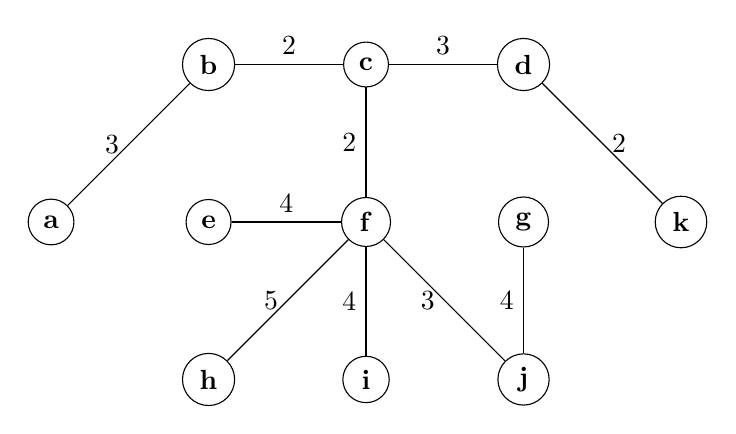
\begin{tikzpicture}
	\node[shape=circle,draw=black] (a) at (0, 2)     {\textbf{a}};
	\node[shape=circle,draw=black] (b) at (2, 4)     {\textbf{b}};
	\node[shape=circle,draw=black] (c) at (4, 4)     {\textbf{c}};
	\node[shape=circle,draw=black] (d) at (6, 4)     {\textbf{d}};
	\node[shape=circle,draw=black] (e) at (2, 2)     {\textbf{e}};
	\node[shape=circle,draw=black] (f) at (4, 2)     {\textbf{f}};
	\node[shape=circle,draw=black] (g) at (6, 2)     {\textbf{g}};
	\node[shape=circle,draw=black] (h) at (2, 0)     {\textbf{h}};
	\node[shape=circle,draw=black] (i) at (4, 0)     {\textbf{i}};
	\node[shape=circle,draw=black] (j) at (6, 0)     {\textbf{j}};
	\node[shape=circle,draw=black] (k) at (8, 2)     {\textbf{k}};

	\path[-] (a) edge node[left]{3} (b);
	\path[-] (b) edge node[above]{2} (c);
	\path[-] (e) edge node[above]{4} (f);
    \path[-] (h) edge node[left]{5} (f);	
	\path[-] (c) edge node[above]{3} (d);
	\path[-] (c) edge node[left]{2} (f);
	\path[-] (f) edge node[left]{3} (j);
    \path[-] (f) edge node[left]{4} (i);
	\path[-] (d) edge node[right]{2} (k);
	\path[-] (g) edge node[left]{4} (j);

	\end{tikzpicture} 
	\caption{A minimum spanning tree}
\end{figure}
\pagebreak
\section*{Answer 6}
\subsection*{a)}
\textbf{Vertices:} 7\\
\textbf{Edges:} 6\\
\textbf{Height:} 4
\subsection*{b)}
$a,b,c,d,e,f,g$
\subsection*{c)}
$b,d,f,g,e,c,a$
\subsection*{d)}
$b,a,d,c,f,e,g$
\subsection*{e)}
Since all internal nodes ($a$, $c$, and $e$) have exactly two children, $T$ is a full binary tree.
\subsection*{f)}
Since level difference between some leaves are more than 1 ($b$ is in level-1, and $f$ is in level-3), $T$ is not a complete binary tree.
\subsection*{g)}
Consider subtree $T_c$ whose root is $c$, and subtree $T_e$, whose root is $e$. $e$ is the right child of $e$, therefore, all vertices of $T_e$ should succeed $c$. Since $f$ is in $T_e$ and, $24 \not\leq 23$. $T_c$ is not a binary search tree. Therefore, $T$ is not a binary search tree.
\subsection*{h)}
Consider a full tree with height 5 in which each internal node has a leaf as its left child, and a full tree as its right child. There are two nodes in each level except level-0, which has only one node, that is the root. Therefore the minimum number of nodes for a full binary tree with height is $1 + 2 + 2 + 2 + 2 + 2 = 11$.
    
\subsection*{i)}

\begin{figure}[H]
    \centering
    \begin{tikzpicture}

        \node[shape=circle,draw=black,minimum size=10mm] (a) at (0, 0) {\textbf{1}};
        \node[shape=circle,draw=black,minimum size=10mm] (b) at (2, 2) {\textbf{2}};
        \node[shape=circle,draw=black,minimum size=10mm] (c) at (4, 0) {\textbf{3}};
        \node[shape=circle,draw=black,minimum size=10mm] (d) at (5, 4) {\textbf{4}};
        \node[shape=circle,draw=black,minimum size=10mm] (e) at (6, 0) {\textbf{5}};
        \node[shape=circle,draw=black,minimum size=10mm] (f) at (8, 2) {\textbf{6}};
        
        \path[-] (d) edge (b);
        \path[-] (d) edge (f);
        \path[-] (b) edge (a);
        \path[-] (b) edge (c);
        \path[-] (f) edge (e);
        
    \end{tikzpicture}
\end{figure}

\subsection*{j)}
\textbf{1:} $4-2-1$\\
\textbf{6:} $4-6$
\subsection*{k)}
\begin{figure}[H]
    \centering
    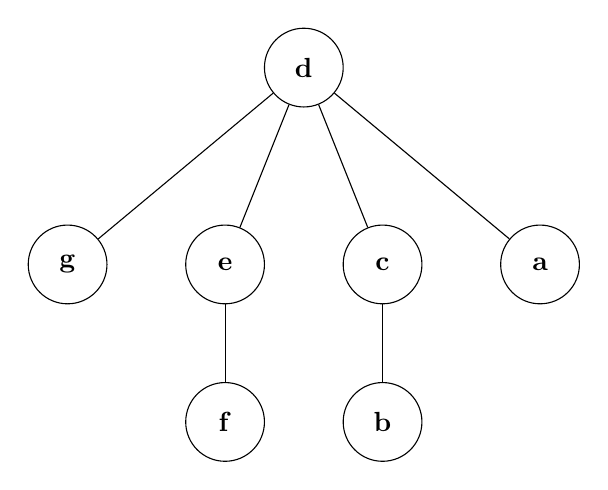
\begin{tikzpicture}

        \node[shape=circle,draw=black,minimum size=10mm] (a) at (6,2) {\textbf{a}};
        \node[shape=circle,draw=black,minimum size=10mm] (b) at (4,0) {\textbf{b}};
        \node[shape=circle,draw=black,minimum size=10mm] (c) at (4,2) {\textbf{c}};
        \node[shape=circle,draw=black,minimum size=10mm] (d) at (3,4.5) {\textbf{d}};
        \node[shape=circle,draw=black,minimum size=10mm] (e) at (2,2) {\textbf{e}};
        \node[shape=circle,draw=black,minimum size=10mm] (f) at (2,0) {\textbf{f}};
        \node[shape=circle,draw=black,minimum size=10mm] (g) at (0,2) {\textbf{g}};

        \path[-] (d) edge (g);
        \path[-] (d) edge (e);
        \path[-] (d) edge (c);
        \path[-] (d) edge (a);
        \path[-] (e) edge (f);
        \path[-] (c) edge (b);

        
    \end{tikzpicture}
    
\end{figure}
\subsection*{l)}
If the least element of the tree is the root of the tree and and its child subtrees, each internal node will have only one child. Therefore, the maximum height is $k-1$.
\end{document}

​

